%beamer

%\PassOptionsToClass{handout}{beamer}

% \newboolean{handoutmode}
% \setboolean{handoutmode}{false}
%\newcommand{\handoutmode}{}

%% LaTeX-Beamer template for KIT design
%% by Erik Burger, Christian Hammer
%% title picture by Klaus Krogmann
%%
%% version 2.1
%%
%% mostly compatible to KIT corporate design v2.0
%% http://intranet.kit.edu/gestaltungsrichtlinien.php
%%
%% Problems, bugs and comments to
%% burger@kit.edu
\ifdefined \handoutmode
\documentclass[18pt, handout]{beamer}
\else
\documentclass[18pt]{beamer}
\fi

\usepackage[T1]{fontenc}
\usepackage[utf8]{inputenc}

\usepackage{../preamble/templates/beamerthemekit}

\usepackage[vlined]{algorithm2e}  %possible: noend, noline, ...
\usepackage{amssymb}
\usepackage{amsmath}
\usepackage{wasysym}
\usepackage{graphicx}
%\usepackage{hyperref}
\usepackage[export]{adjustbox}
\usepackage{wrapfig}
\usepackage{colortbl}
\usepackage{tikz}
\usetikzlibrary{matrix}
\usetikzlibrary{arrows.meta}
\usetikzlibrary{automata}
\usetikzlibrary{tikzmark}
\graphicspath{{images/}}
%\usepackage[colorlinks=true,urlcolor=blue,linkcolor=blue]{hyperref}
\usepackage[outline]{contour}
\usepackage{cancel}
\usepackage[warn]{textcomp}
\usepackage{multicol}
\usepackage{tabularx}
\usepackage{xcolor}
\usepackage{hhline}
\usepackage{environ}
\usepackage{calc}
\usepackage{bm}
\usepackage{xspace} % for \xspace command
\usepackage{varwidth}
\usepackage{csquotes}

\newcommand{\mycomment}[1]{}

%%%% CONFIG

\input{../preamble/config.tex}

%%%% CONFIG END

%\renewcommand{\SS}{\iffontchar\font"1E9E \symbol{"1E9E}\else SS\fi} % SHAME ON YOU, LATEX!
\newcommand{\TM}{\text{$\mbox{}^\text{\tiny TM}$}}
\newcommand{\pluseq}{\mathrel{+}=}
\newcommand{\pp}{\operatorname{++}} 
\newcommand{\mm}{\operatorname{--\mbox{\:}--}}
\newcommand{\minuseq}{\mathrel{-}=}
\newcommand{\asteq}{\mathrel{*}=}
\newcommand{\muleq}{\asteq}
\renewcommand{\mod}{\mathop{\textbf{mod}}} 
\renewcommand{\div}{\mathop{\textbf{div}}}
\newcommand{\N}{\mathbb{N}} 
\newcommand{\R}{\mathbb{R}}
\newcommand{\Z}{\mathbb{Z}}
\newcommand{\E}{\mathbb{E}}
\renewcommand{\P}{\mathbb{P}}
\newcommand{\BB}{\mathbb{B}} % \B already exists
\newcommand{\NP}{\ensuremath{\mathcal{N\hspace{-1.5pt}P}}}
\newcommand{\Oh}[1]{\mathcal{O}\!\left(#1\right)}
\renewcommand{\O}{\mathcal{O}}
\newcommand{\Om}[1]{\Omega\!\left(#1\right)}
\newcommand{\Th}[1]{\Theta\!\left(#1\right)}

\newcommand{\realTilde}{\textasciitilde\xspace}
\renewcommand{\qedsymbol}{\textcolor{black}{\openbox}}

\newcommand{\size}[1]{\ensuremath{\left\lvert #1 \right\rvert}}
\newcommand{\set}[1]{\left\{#1\right\}}
\newcommand{\tuple}[1]{\left(#1\right)}

\newcommand*{\from}{\colon}

\newcommand{\morescalingdelimiters}{   % for proper \left( \right) typography
	\delimitershortfall=0pt  % formerly: 0pt  
	\delimiterfactor=1
}
% todo later
%\delimitershortfall=0pt  % for proper \left( \right) typography
%\delimiterfactor=1

% --- \frameheight constant ---
\newlength\fullframeheight
\newlength\framewithtitleheight
\setlength\fullframeheight{.92\textheight}
\setlength\framewithtitleheight{.86\textheight}

\newlength\frameheight
\setlength\frameheight{\fullframeheight}

\let\frametitleentry\relax
\let\oldframetitle\frametitle
\def\frametitle#1{\global\def\frametitleentry{#1}\if\relax\frametitleentry\relax\else\setlength\frameheight{\framewithtitleheight}\fi\oldframetitle{#1}}

% --- \frameheight constant end ---

\def\·{\cdot}
\def\*{\cdot}
\def\<{\langle}
\def\>{\rangle}


\newcommand{\zB}{z.\,B.\@\xspace}
\newcommand{\ZB}{Z.\,B.\@\xspace}

\newcommand{\ceil}[1]{\left\lceil#1\right\rceil}
\newcommand{\floor}[1]{\left\lfloor#1\right\rfloor}
\newcommand{\abs}[1]{\left|#1\right|}
\newcommand{\Matrix}[1]{\begin{pmatrix} #1 \end{pmatrix}}
\newcommand{\braced}[1]{\left\lbrace #1 \right\rbrace}
\newcommand{\llist}[1]{\langle #1 \rangle}
\newcommand{\Mid}{\;\middle|\;}

\let\after\circ

\newcommand{\entspr}{\ensuremath{\mathrel{\hat{=}}}\xspace}

\def\~~>{\ensuremath{\rightsquigarrow}}  % FuCKING FINALLY! :D

% "something" placeholder. Useful for repairing spacing of operator sections, like `\sth = 42`.
\def\sth{\vphantom{.}}

\def\fract#1/#2 {\frac{#1}{#2}}  % ! TRAILING SPACE is CRUCIAL!
\def\dfract#1/#2 {\dfrac{#1}{#2}} % ! Trailing space is crucial!

\newcommand{\tight}[1]{{\renewcommand{\arraystretch}{0.76} #1}}
\newcommand{\stackedtight}[1]{{\renewcommand{\arraystretch}{0.76} \begin{matrix} #1 \end{matrix}} }
\newcommand{\stacked}[1]{\begin{matrix} #1 \end{matrix} }
\newcommand{\casesl}[1]{\delimitershortfall=0pt  \left\lbrace\hspace{-.3\baselineskip}\begin{array}{ll} #1 \end{array}\right.}
\newcommand{\casesr}[1]{\delimitershortfall=0pt  \left.\begin{array}{ll} #1 \end{array}\right\rbrace}
\newcommand{\caseslr}[1]{\delimitershortfall=0pt  \left\lbrace\begin{array}{ll} #1 \end{array}\hspace{-.3\baselineskip}\right\rbrace}

\def\q#1uad{\ifnum#1=0\relax\else\quad\q{\the\numexpr#1-1\relax}uad\fi}
% e.g. \q1uad = \quad, \q2uad = \qquad etc.

\newcommand{\qqquad}{\q3uad}


\def\indentstring{}
\def\§#1{\def\indentstring{#1}#1}
\def\.{{$\hphantom{\text{\indentstring}}$}}


\newcommand{\impl}{\ifmmode\ensuremath{\mskip\thinmuskip\Rightarrow\mskip\thinmuskip}\else$\Rightarrow$\xspace\fi}  
\newcommand{\Impl}{\ifmmode\implies\else$\Longrightarrow$\xspace\fi}

\newcommand{\gdw}{\ifmmode\mskip\thickmuskip\Leftrightarrow\mskip\thickmuskip\else$\Leftrightarrow$\xspace\fi}
\newcommand{\Gdw}{\ifmmode\iff\else$\Longleftrightarrow$\xspace\fi}

\newcommand{\symbitemnegoffset}{\hspace{-.33\baselineskip}}
\newcommand{\implitem}{\item[\impl\symbitemnegoffset]}
\newcommand{\Implitem}{\item[\Impl\symbitemnegoffset]}


\newcommand{\forcenewline}{\mbox{}\\}

\newcommand{\bfalert}[1]{\textbf{\alert{#1}}}
\let\elem\in   % I'm a Haskell freak. Don't judge me. :P


\newenvironment{threealign}{%
	\[
	\begin{array}{r@{\ }c@{\ }l}
}{%
	\end{array}	
	\]
}


\makeatletter
% Provides color if undefined.
\newcommand{\colorprovide}[2]{%
	\@ifundefinedcolor{#1}{\colorlet{#1}{#2}}{}}
\makeatother



%\pgfdeclarelayer{background}
%\pgfdeclarelayer{foreground}
%\pgfsetlayers{background,main,foreground}

\colorprovide{lightred}{red!30}
\colorprovide{lightgreen}{green!40}
\colorprovide{lightyellow}{yellow!50}
\colorprovide{beamerlightred}{lightred}
\colorprovide{beamerlightgreen}{lightgreen}
\colorprovide{beamerlightyellow}{lightyellow}
\colorprovide{fullred}{red!60}
\colorprovide{fullgreen}{green}
\definecolor{darkred}{RGB}{115,48,38}
\definecolor{darkgreen}{RGB}{48,115,38}
\definecolor{darkyellow}{RGB}{100,100,0}

\only<handout:0>{\colorlet{adaptinglightred}{beamerlightred}}
\only<handout:0>{\colorlet{adaptinglightgreen}{beamerlightgreen}}
\only<handout:0>{\colorlet{adaptinglightyellow}{beamerlightyellow}}
\only<beamer:0>{\colorlet{adaptinglightred}{lightred}}
\only<beamer:0>{\colorlet{adaptinglightgreen}{lightgreen}}
\only<beamer:0>{\colorlet{adaptinglightyellow}{lightyellow}}
\only<handout:0>{\colorlet{adaptingred}{lightred}}
\only<beamer:0>{\colorlet{adaptingred}{fullred}}
\only<handout:0>{\colorlet{adaptinggreen}{lightgreen}}
\only<beamer:0>{\colorlet{adaptinggreen}{fullgreen}}

\colorlet{checkgreen}{green!80}
\colorlet{crashred}{fullred}
\colorprovide{myalertcolor}{red}
\colorlet{alertcolor}{myalertcolor}

\definecolor{kwblue}{rgb}{0.3,0.3,1}
\definecolor{strcolor}{RGB}{48,115,38}

\newcommand{\str}[1]{\shorthandoff{"}\textcolor{strcolor}{\text{"{}#1"{}}\shorthandon{"}}}

\newcommand{\gray}[1]{\textcolor{gray}{#1}}

\newcommand{\MyKwSty}[1]{\textcolor{kwblue}{\textbf{#1}}}
\SetKwSty{MyKwSty}

\SetArgSty{textnormal} % to end conditional italics madness

\newcommand{\MyCommentSty}[1]{\emph{\gray{#1}}}
\SetCommentSty{MyCommentSty}

\SetKwComment{Comment}{// }{}

\newcommand{\LComment}[1]{\Comment*[h]{#1}}
\newcommand{\RComment}[1]{\quad \Comment*[h]{#1}}



\SetKwBlock{KwFunc}{function}{}
\SetKwBlock{KwProc}{procedure}{}
\newcommand{\Function}[2]{\KwFunc({#1}){#2}}
\newcommand{\Procedure}[2]{\KwProc({#1}){#2}}
\SetKwBlock{KwEmptyBlock}{}{}
\newcommand{\EmptyBlock}[1]{\KwEmptyBlock(){#1}}

% Binary operator keywords (small surrounding spaces)
\newcommand{\SetKwBin}[2]{
	\expandafter\newcommand\csname #1\endcsname{\ensuremath{\mathbin{\KwSty{#2}}}}	
}
% Relational operator keywords (bigger surrounding spaces)
\newcommand{\SetKwRel}[2]{
	\expandafter\newcommand\csname #1\endcsname{\ensuremath{\mathrel{\KwSty{#2}}}}	
}
% Directive keywords (trailing space)
\newcommand{\SetKwDir}[2]{
	\expandafter\newcommand\csname #1\endcsname{\ensuremath{\mathop{\KwSty{#2}}}}		
}

\DontPrintSemicolon
%\SetKwSwitch{Switch}{Case}{Other}{switch on}{}{}{else}{}{}

%\newcommand{\SwitchCase}[2]{\KwSty{case} #1 \KwOf\EmptyBlock{#2}}
%\newcommand{\case}[2]{#1:\EmptyBlock{#2}}
\SetKwDir{KwAssert}{assert}
\SetKwDir{KwInvariant}{invariant}
\SetKwRel{KwStep}{step}
\SetKwRel{KwDownto}{downto}	
\SetKwDir{KwArrayOf}{array of\,}
\SetKwDir{KwArray}{array}
\let\KwTo\undefined
\SetKwRel{KwTo}{to}
\SetKwRel{KwOf}{of}
\let\KwInput\KwIn
\let\KwIn\undefined
\SetKwRel{KwIn}{in}
\SetKwRel{KwInto}{into}
\SetKwDir{KwNot}{not}
\SetKwRel{KwIs}{is}
\SetKwRel{KwAnd}{and}
\SetKwRel{KwOr}{or}
\SetKwBin{KwMod}{mod}
\SetKwBin{KwDiv}{div}
\SetKwDir{KwContinue}{continue}
\SetKwDir{KwBreak}{break}
\SetKwDir{KwThrow}{throw}
\SetKw{KwTrue}{true}
\SetKw{KwFalse}{false}
\SetKw{KwThis}{this}
\SetKwDir{KwNew}{new}
\SetKwRel{KwFrom}{from}
\SetKwDir{KwFor}{for}
\SetKwDir{KwEach}{each}
\SetKw{KwProcedure}{procedure}
\SetKw{KwMethod}{method}
\SetKw{KwFunction}{function}
\SetKwDir{KwPointerTo}{Pointer to}
\SetKwData{KwList}{List}
\SetKwData{KwSet}{Set}
\newcommand{\Element}{\|Element|}
\newcommand{\KwListOf}{\ensuremath{\mathop{\KwList \KwOf}}} 
\newcommand{\KwSetOf}{\ensuremath{\mathop{\KwSet \KwOf}}} 
\SetKwDir{KwDispose}{dispose}


\def\|#1|{\text{\normalfont #1}}  % | steht für senkrecht (anstatt kursiv wie sonst im math mode)

% proper math typography
\newcommand{\functionto}{\longrightarrow} 
\renewcommand{\geq}{\geqslant}
\renewcommand{\leq}{\leqslant}
\let\oldsubset\subset
\renewcommand{\subset}{\subseteq} % for all idiots out there using subset

\newcommand{\access}{\text{\textrightarrow}} 
\def\->{\access}

\let\oldemptyset\emptyset
\let\emptyset\varnothing % proper emptyset

\newcommand{\stdarraystretch}{1.20}
\renewcommand{\arraystretch}{\stdarraystretch}  % for proper row spacing in tables

\newcommand{\mailto}[1]{\href{mailto:#1}{{\textcolor{blue}{\underline{#1}}}}}
\newcommand{\urlnamed}[2]{\href{#1}{\textcolor{blue}{\underline{#2}}}}
\renewcommand{\url}[1]{\urlnamed{#1}{#1}}

\newcommand{\hanging}{\hangindent=0.7cm}
\newcommand{\indented}{\hanging}

\newcommand{\Pros}{{\huge \protect\textcolor{adaptinggreen}{\protect\contour{black}{\raisebox{-.3pt}{$\protect\textbf{+}$}}}}\xspace}

\newcommand{\Cons}{\hspace{1pt}\protect\scalebox{0.88}[1]{\huge \protect\contour{black}{\protect\textcolor{adaptingred}{\raisebox{-1pt}{$\protect\textbf{--}$}}}}\hspace{1pt}\xspace}

\newcommand{\yop}{\textcolor{checkgreen}{\protect\contour{black}{\protect\textbf{\checked}}}\xspace}
\newcommand{\crash}{\ensuremath{\textcolor{crashred}{\protect\contour{black}{\protect\textbf{\lightning}}}}\xspace}

\newcommand{\YesCellE}[1]{\cellcolor{adaptinggreen} {#1}}
\newcommand{\YesCell}{\YesCellE{\textbf{Ja}}}
\newcommand{\NoCellE}[1]{\cellcolor{adaptingred} {#1}}
\newcommand{\NoCell}{\NoCellE{\textbf{Nein}}}


\newcommand{\TrueQuestion}[1]{
	\TrueQuestionE{#1}{}
}

\newcommand{\YesQuestion}[1]{
	\YesQuestionE{#1}{}
}

\newcommand{\FalseQuestion}[1]{
	\FalseQuestionE{#1}{}
}

\newcommand{\NoQuestion}[1]{
	\NoQuestionE{#1}{}
}

\newcommand{\DependsQuestion}[1]{
	\DependsQuestionE{#1}{}
}

\newcommand{\QuestionVspace}{\vspace{4pt}}
\newcommand{\QuestionParbox}[1]{\begin{varwidth}{.85\linewidth}#1\end{varwidth}}
\newcommand{\ExplanationParbox}[1]{\begin{varwidth}{.99\linewidth}#1\end{varwidth}}
\colorlet{questionlightgray}{gray!23}
\let\defaultfboxrule\fboxrule

% #1: bg color
% #2: fg color short answer
% #3: short answer text
% #4: question
% #5: explanation
\newcommand{\GenericQuestion}[5]{
	\setlength\fboxrule{2pt}
	\only<+|handout:0>{\hspace{-2pt}\fcolorbox{white}{questionlightgray}{\QuestionParbox{#4} \quad\textbf{?}}}
	\visible<+->{\hspace{-2pt}\fcolorbox{white}{#1}{\QuestionParbox{#4} \quad\textbf{\textcolor{#2}{#3}}} \ExplanationParbox{#5}} \\
	\setlength\fboxrule{\defaultfboxrule}
}

% #1: Q text
% #2: Explanation
\newcommand{\TrueQuestionE}[2]{
	\GenericQuestion{adaptinglightgreen}{darkgreen}{Wahr.}{#1}{#2}
}

% #1: Q text
% #2: Explanation
\newcommand{\YesQuestionE}[2]{
	\GenericQuestion{adaptinglightgreen}{darkgreen}{Ja.}{#1}{#2}
}

% #1: Q text
% #2: Explanation
\newcommand{\FalseQuestionE}[2]{
	\GenericQuestion{adaptinglightred}{darkred}{Falsch.}{#1}{#2}
}

% #1: Q text
% #2: Explanation
\newcommand{\NoQuestionE}[2]{
	\GenericQuestion{adaptinglightred}{darkred}{Nein.}{#1}{#2}
}

% #1: Q text
% #2: Explanation
\newcommand{\DependsQuestionE}[2]{
	\GenericQuestion{adaptinglightyellow}{darkyellow}{Je nachdem!}{#1}{#2}
}

\newenvironment{headframe}{\Huge THIS IS AN ERROR. PLEASE CONTACT THE ADMIN OF THIS TEX CODE. (headframe env def failed)}{}
\RenewEnviron{headframe}[1][]{
	\begin{frame}\frametitle{\ }
		\centering 
		\Huge\textbf{\textsc{\BODY} \\
		} 
		\Large {#1}
		\frametitle{\ }
	\end{frame}
}

\newcommand{\sectionheadframe}[2]{
	\section{#1}
	\begin{headframe}[#2]
		#1
	\end{headframe}	
}

\newcommand{\slideThanks}{
	\begin{frame}{Credits}
		%\begin{block}{}
			Vorgänger dieses Foliensatzes wurden erstellt von: \\[1em]
			Christopher Hommel  (urspr. Verfasser)\\
			Daniel Jungkind 
		%\end{block}
	\end{frame}
}

%% SLIDE FORMAT

% use 'beamerthemekit' for standard 4:3 ratio
% for widescreen slides (16:9), use 'beamerthemekitwide'


% \usepackage{../preamble/templates/beamerthemekitwide}

%% TITLE PICTURE

% if a custom picture is to be used on the title page, copy it into the 'logos'
% directory, in the line below, replace 'mypicture' with the 
% filename (without extension) and uncomment the following line
% (picture proportions: 63 : 20 for standard, 169 : 40 for wide
% *.eps format if you use latex+dvips+ps2pdf, 
% *.jpg/*.png/*.pdf if you use pdflatex)
\IfFileExists{images/logo.png}{
	\titleimage{logo}
}{}
\IfFileExists{images/logo.jpg}{
	\titleimage{logo}
}{}

%% TITLE LOGO

% for a custom logo on the front page, copy your file into the 'logos'
% directory, insert the filename in the line below and uncomment it

\titlelogo{empty}

% (*.eps format if you use latex+dvips+ps2pdf,
% *.jpg/*.png/*.pdf if you use pdflatex)

%% TikZ INTEGRATION

% use these packages for PCM symbols and UML classes
% \usepackage{templates/tikzkit}
% \usepackage{templates/tikzuml}

% the presentation starts here


%% Titel einfügen
\newcommand{\titleframe}{\frame{\titlepage}}

\newcounter{weeknum}

\newcounter{tasknum}
\newcounter{subtasknum}
\resetcounteronoverlays{subtasknum}
\resetcounteronoverlays{tasknum}
\let\oldthesubtasknum\thesubtasknum
\def\thesubtasknum{\ifnum\oldthesubtasknum=0\relax\else\alph{subtasknum})\fi}
\def\ThisHasSubtasks{\setcounter{subtasknum}{1337}}
\def\thetasknumminusone{\the\numexpr\thetasknum-1\relax\xspace}
\newcommand{\taskheading}[1]{\ifnum\oldthesubtasknum=1337\relax\setcounter{subtasknum}{1}\else\setcounter{subtasknum}{0}\fi\addtocounter{tasknum}{1}\textbf{Aufgabe \thetasknum\thesubtasknum: #1} \\}
\newcommand{\subtaskheading}[1]{\addtocounter{subtasknum}{1}\textbf{Aufgabe \thetasknum\thesubtasknum: #1} \\}
\newcommand{\solutionheading}{\textbf{Lösung zu Aufgabe \thetasknum\thesubtasknum} \\}

\setbeamertemplate{section in toc}{
	\gray{\inserttocsection} \par	
}
\setbeamertemplate{navigation symbols}{}

\newif\ifprinttableofcontents \printtableofcontentstrue
\def\notableofcontents{\printtableofcontentsfalse}
\let\notoc\notableofcontents

%% Alles starten mit \starttut{X}
\newcommand{\starttut}[1]{\setcounter{weeknum}{#1}\pdfinfo{
		/Author (\myname)
		/Title  (Algorithmen-Tutorium \mytutnumber, Woche \theweeknum)
	}\titleframe
	\ifprinttableofcontents\frame{\frametitle{Inhalt}\tableofcontents}\fi
	\mycomment{
		\AtBeginSection[]{%
			\begin{frame}{Wo sind wir gerade?}
				\tableofcontents[currentsection]
			\end{frame}\addtocounter{framenumber}{-1}
		}
	}	
}


\newcommand{\framePrevEpisode}{
	\begin{headframe}
		\mylasttimestext
	\end{headframe}
}

\newcommand{\lastframetitled}[6]{
	\frame{\frametitle{#6}
		\vspace{-#2\baselineskip}
		\begin{figure}[H]
			\centering
			\LARGE \textbf{\textsc{#5}} \\
			\vspace{.2\baselineskip}
			\includegraphics[#1]{#3}
			\vspace{-10pt}
			\begin{center}
				\small \url{#4} 
			\end{center}
		\end{figure} 
	}
}

% #1 number
% #2 title 
% #3 vspace (positive) without unit (\baselineskip)
\newcommand{\xkcdframe}[3]{
	\lastframetitled{width=.96\textwidth}{#3}{xkcd_#1}{http://xkcd.com/#1}{}{#2}
}

\newcommand{\xkcdframevert}[3]
{
	\lastframetitled{height=.96\frameheight}{#3}{xkcd_#1}{http://xkcd.com/#1}{}{#2}
}

\newif\ifisWS \isWSfalse

\def\semesterWS{\isWStrue}
\def\semesterSS{\isWSfalse}

\semesterSS

\def\semesterstring{\ifisWS WS \thisyear/\the\numexpr\nextyear-2000\relax\else SS \thisyear\fi}

\edef\nextyear{\the\numexpr\thisyear+1\relax} 

\title[Algorithmen-Tutorium \mytutnumber, Woche \theweeknum]{Algorithmen I \\[-2pt] Tutorium \mytutnumber}
\subtitle{Woche \theweeknum\ |\xspace\mydate{\theweeknum}}


\author[\myname]{{\mynamebold \; (\mailto{\mymail})}}

\institute{Institut für Theoretische Informatik}

\date{\mydate{\theweeknum}\ }



% Bibliography
% not needed here:
%\usepackage[citestyle=authoryear,bibstyle=numeric,hyperref,backend=biber]{biblatex}
%\addbibresource{templates/example.bib}
%\bibhang1em

% presentation

\setbeamercovered{transparent=1}  %min=0, max=100

% change the following line to "ngerman" for German style date and logos
\selectlanguage{ngerman}

\ifnum\thisyear=2018 \else \errmessage{Old ILIAS link inside preamble. Please update.} \fi

\newcommand{\ILIAS}{\urlnamed{https://ilias.studium.kit.edu/ilias.php?ref_id=808428&cmdClass=ilrepositorygui&cmdNode=k8&baseClass=ilrepositorygui}{ILIAS}\xspace} 

\newcommand{\Socrative}{\only<handout:0>{socrative.com $\qquad$ \~~> Student login \\ Raumname:  \mysocrativeroom\\ \medskip}}

\newcommand{\thasse}[1]{
	\ifdefined\ThassesTut #1\xspace \else\fi
}
\newcommand{\daniel}[1]{
	\ifdefined\DanielsTut #1\xspace \else\fi
}
\newcommand{\thassedaniel}[2]{\ifdefined\ThassesTut #1\else\ifdefined\DanielsTut #2\fi\fi\xspace}

\ifdefined\ThassesTut \ifdefined\DanielsTut \errmessage{ERROR: Both ThassesTut and DanielsTut flags are set. This is most likely an error. Please check your config.tex file.} \else \fi \else \ifdefined\DanielsTut \else \errmessage{ERROR: Neither ThassesTut  nor DanielsTut flags are set. This is most likely an error. Please check your config.tex file.} \fi\fi

\morescalingdelimiters

\begin{document}
	
\starttut{10}
	


\begin{headframe}[Es kommt halt \textit{doch} auf die Länge an...]
	Kürzeste Pfade
\end{headframe}
	
\begin{frame}{Kürzeste Pfade – Dijkstra}
	\textbf{Der unaussprechliche Algorithmus} 
	\begin{itemize}
		\item \underline{Gesucht}: \textbf{Kürzeste gewichtete} Pfade \\
		von Startknoten $s \in V$ zu \textbf{allen} anderen Knoten
		\pause
		\item \textit{Breitensuche}: Findet kürzeste Pfade bei \textbf{ungewichteten} Kanten
		\pause
		\implitem Passe BFS für gewichtete Kanten an, \\
		verwende zwei $\KwArray$s:
		\begin{itemize}
			\item $d[v]$: Länge des \textbf{bisher bekannten} kürzesten Pfades zu $v$ 
			\vspace{.2\baselineskip}
			\item $parent[v]$: \textbf{Direkter} Vorgänger von $v$ im \textbf{bisher bekannten} kürzesten Pfad zu $v$
		\end{itemize}
		\pause
		\item Rüste Queue $Q$ auf zu einer \textbf{PriorityQueue} $PQ$ (z.B. binärer Heap), Knoten $v$ wird mit $d[v]$ gewichtet
		%\pause
		%\item Invariante: Kürzester Pfad zu $PQ.min$ ist bekannt
		\pause
		\item Wichtige Einschränkung: \textbf{Keine negativen Kantengewichte!}
	\end{itemize}
\end{frame}

\begin{frame}{Kürzeste Pfade – Dijkstra}  \vspace{-.25\baselineskip}
	\begin{exampleblock}{} \vspace{-.4\baselineskip}
		\begin{algorithm}[H]
			\small
			\Function {Dijkstra$(G = (V, E),\ s \in V)$} {
				$d := (\infty, ..., \infty) : \KwArray[1...n] \KwOf \R$\;
				$parent := (\bot, .., \bot) : \KwArray[1...n] \KwOf V$\;
				$PQ = \{s\} : $ PriorityQueue\;
				$parent[s] := s, \quad d[s] := 0$ \;
				\While{$PQ \neq \emptyset$} {
					$u := PQ.$deleteMin$()$ \RComment{u wird jetzt „gescannt“} \;
					\ForEach(\RComment{„Relaxiere“ e}){$e = (u, v) \in E$} {
						\If{$d[u] + c(e) < d[v]$} {
							$d[v] := d[u] +c(e)$\;
							$parent[v] := u$\;
							\eIf{$v \in PQ$} {
								$PQ.$decreaseKey$(v)$\;
							}{
							$PQ.$insert$(v)$\;
							}
						}
					}
				}
				\Return{$(d, parent)$}\;
			}
		\end{algorithm}
	\end{exampleblock}
\end{frame}

\begin{frame}{Kürzeste Pfade – Dijkstra}
	\textbf{Korrektheit}
	\begin{itemize}
		%\pause
		\item \textbf{Invariante}: Wenn ein Knoten aus $PQ$ entnommen wird, ist zu diesem der \textbf{endgültige} kürzeste Pfad bekannt
		\pause
		\item Beweis der Invariante durch \textbf{vollständige Induktion} über die Schleifendurchläufe möglich
	\end{itemize}
\end{frame}

\iffalse

\begin{frame}{Kürzeste Pfade – Dijkstra}
	\textbf{Korrektheitsbeweis} \\
	%\begin{itemize}
	%\pause
	\underline{IA.:} Endgültiger kürzester Pfad zu $s$: Trivial \yop \\[0,125cm]
	\pause
	\underline{IV.:} Zu allen Knoten $v_1, ..., v_{i-1}$, die aus der $PQ$ entnommen wurden, \\
	\quad\ \ ist der \textbf{endgültige} kürzeste Pfad bekannt \\[0,125cm]
	\pause
	\underline{IS.:} Knoten $v_i$ wird entnommen. Der bekannte kürzeste Pfad führt \\
	\quad\ \ „irgendwie“ über $v_1 ... v_{i-1}$ zu $v_i$. \\
	\pause
	\quad\ \ Ang., es gibt einen \textbf{echt} kürzeren Pfad zu $v_i$. Dieser \textbf{muss} dann über \\
	\quad\ \ einen Knoten $p$ aus der $PQ$ zu $v_i$ führen. \\
	\pause
	\quad\ \ Dafür gibt es zwei Möglichkeiten: \\
	\pause
	\quad\ \ Fall 1: Zu $p$ gibt es einen kürzeren Pfad als zu $v_i$ \\
	\pause
	\qquad\qquad\ \ \impl $p$ wurde \textbf{vor} $v_i$ aus der $PQ$ entnommen \crash \\
	\pause
	\quad\ \ Fall 2: Der Pfad über $p$ zu $v_i$ ist kürzer als der kürzeste Pfad zu $p$ \\
	\pause
	\qquad\qquad\ \ \impl $c((p, v_i)) < 0$ \crash { \small(Keine negativen Kantengewichte erlaubt!)}
	%\end{itemize}
\end{frame}

\begin{frame}{Kürzeste Pfade – Dijkstra}
	\textbf{Korrektheitsbeweis} \\
	\begin{itemize}
		\item \textbf{Terminierung}: In \textbf{jedem} Schleifendurchlauf wird ein Knoten $v$ aus $PQ$ entnommen. Da dann der \textbf{endgültige} kürzeste Pfad zu $v$ bekannt ist, wird $v$ danach \textbf{nicht} mehr erneut in die $PQ$ eingefügt \\
		\impl Nach maximal $n$ Schleifendurchläufen ist $PQ$ leer und der Algorithmus terminiert.
	\end{itemize}
\end{frame}

\fi

\begin{frame}{Kürzeste Pfade – Dijkstra}
	\textbf{Laufzeit von Dijkstra} 
	\begin{itemize}
		\item[] Im Worst-Case $m$-mal $decreaseKey$
		\item[$+$] Genau $n$-mal $deleteMin$ und $insert$
		\pause
		\item[$=$] Mit binärem Heap: $O\left((m+n)\log n\right)$
		\pause
		\item[$=$] Mit Fibonacci-Heap: $O(m + n \log n)$ \quad (amortisiert und mit höheren konstanten Faktoren)
	\end{itemize}
\end{frame}

\begin{frame}{Kürzeste Pfade}
	\underline{Aufgabe 1: Noch kürzere kürzeste Pfade} \\
	Gegeben sei ein ( gerichteter oder ungerichteter) zusammenhängender Graph $G = (V, E)$ mit nichtnegativen Kantengewichten $\omega : E \functionto \R^{+}$. Beschreibt einen effizienten Algorithmus, der für einen Startknoten $s$ und alle Zielknoten $t \in V$ den Pfad mit den \textbf{wenigsten} Kanten unter allen kürzesten Pfaden von $s$ nach $t$ berechnet.
\end{frame}

\begin{frame}{Kürzeste Pfade}
	\underline{Lösung zu Aufgabe 1} \\
	\textbf{Modifiziere} Dijkstra: Definiere Kantengewichte um als \textbf{Tupel} $c'(e) := \left(c(e), 1\right)$ (mit komponentenweiser Addition) und folgender Ordnung: \\ $(a, b) < (c, d) \Gdw a < c \ \lor\  (a = c \land b < d)$ 
\end{frame}

\begin{frame}{Kürzeste Pfade – Bellman-Ford}
	\textbf{Rohe Gewalt: Bellman-Ford} 
	\begin{itemize}
		\pause
		\item \textbf{Problem}: Dijkstra „erstickt“ an negativen Kantengewichten
		\pause
		\item \textbf{Überlegung}: Längster (zyklenfreier) Pfad hat \textbf{maximal} $n-1$ Kanten
		\pause
		\implitem Relaxiere jede Kante $(n-1)$-mal \impl \textbf{jeder} minimale zyklenfreie Pfad wurde bestimmt
		\pause
		\item \textbf{Laufzeit}: $O(n \cdot m)$
	\end{itemize}
\end{frame}

\begin{frame}{Kürzeste Pfade – Bellman-Ford}
	\begin{exampleblock}{}
		\begin{algorithm}[H]
			\small
			\Function {BellmanFord$(G = (V, E),\ s \in V)$} {
				$d := (\infty, ..., \infty) : \KwArray[1...n] \KwOf \R$\;
				$parent := (\bot, ..., \bot) : \KwArray[1...n] \KwOf V$\;
				$parent[s] := s ; \quad d[s] := 0$ \;
				\KwSty{do} $n-1$ \KwSty{times} \EmptyBlock{
					\ForEach{$e = (u, v) \in E$} {
						\If{$d[u] + c(e) < d[v]$} {
							$d[v] := d[u] + c(e)$\;
							$parent[v] := u$\;
						}
					}
				}
				\ForEach{$e = (u, v) \in E$} {
					\If{$d[u] + c(e) < d[v]$} {
						\LComment{kleinerer zyklenfreier Pfad ist nicht möglich \impl Negativer Zyklus}
						$d[v] := -\infty$\;
					}
				}
				\KwRet{$(d, parent)$}\;
			}
		\end{algorithm}
	\end{exampleblock}
\end{frame}



\begin{frame}{Graphen}
	\underline{Aufgabe 2: Der Klassiker} \\
	Ein Fährmann soll einen Wolf, eine Ziege und einen Kohlkopf von der linken auf die rechte Seite eines Flusses befördern. Sein kleines Boot hat aber nur Platz für ihn und ein weiteres Objekt. \\
	Außerdem frisst der Wolf die Ziege und die Ziege den Kohlkopf, wenn der Fährmann nicht dabei ist. Zum Glück mag der Wolf kein Gemüse. Wie kann der Fährmann den Wolf, die Ziege und den Kohlkopf unbeschadet übersetzen? \\
	Löst das Problem mithilfe eines Graphen zeichnerisch.
\end{frame}

\begin{frame}{Graphen}
	\underline{Lösung zu Aufgabe 2} \\
	Ein Zustandsgraph: \\
	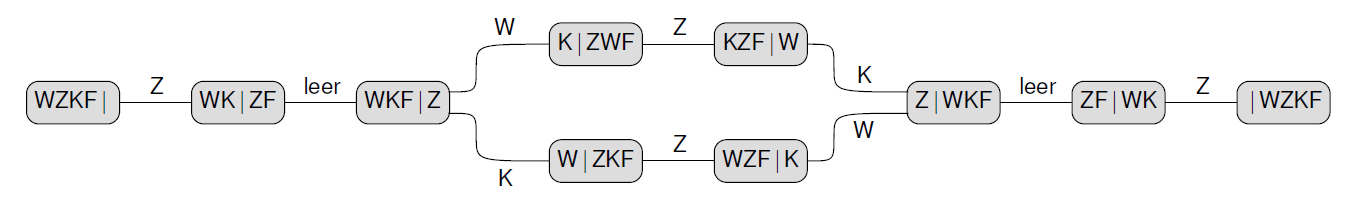
\includegraphics[width=1.03\textwidth]{faehrmann} \\
	Weg von [WZKF|] nach [|WZKF] ist Lösung.
\end{frame}

\begin{frame}{Graphen}
	\underline{Aufgabe 3: Domino Day} \\
	Ihr habt folgende Dominosteine gegeben: \\
	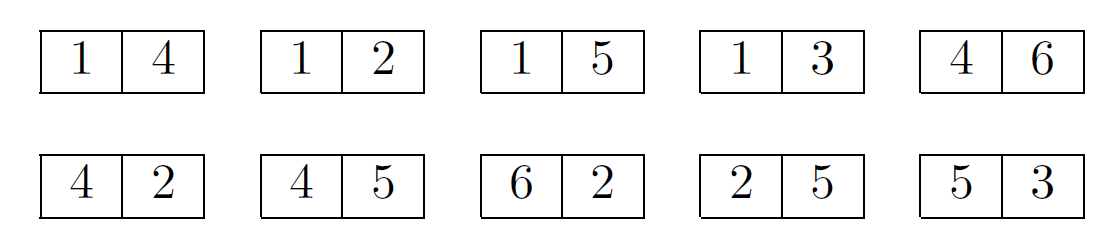
\includegraphics[width=.7\textwidth]{domino-aufg} \\
	Ist es möglich, alle Steine als einen geschlossenen Ring anzuordnen, sodass nur gleiche Zahlen aneinanderliegen? Löst das Problem mithilfe eines Graphen zeichnerisch.
\end{frame}

\begin{frame}{Graphen}
	\underline{Lösung zu Aufgabe 3} \\
	Pro Zahl ein Knoten, pro Stein eine Kante zwischen zwei Knoten. \\
	Zyklus $1 \rightarrow 4 \rightarrow 6 \rightarrow 2 \rightarrow 5 \rightarrow 3 \rightarrow 1 \rightarrow 2 \rightarrow 4 \rightarrow 5 \rightarrow 1$ ist Lösung. \\
	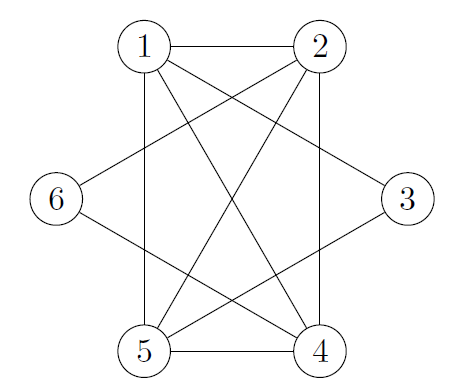
\includegraphics[width=.4\textwidth]{domino-lsg} \\
	\pause
	Allgemein lösbar, wenn Graph zusammenhängend ist und eulerschen Kreis enthält (\gdw nur gerade Knotengrade enthält). \\
	{\small (siehe Exkurs nächste Folie)}
\end{frame}

\begin{frame}{Exkurs Eulerkreis/Hamiltonkreis}
	\textbf{Eulerkreis}: \\
	Kreis, der jede \textbf{Kante} genau einmal beschreitet. {\small (\textbf{E}uler \impl \textbf{E}dges \impl Kanten)} \\
	\forcenewline
	\pause
	\textbf{Hamiltonkreis}: \\
	Kreis, der jeden \textbf{Knoten} genau einmal beschreitet. \\
	\forcenewline
	\pause
	$\exists$ Eulerkreis in $G$ \gdw $G$ hat nur gerade Knotengrade. \\
	$\exists$ Hamiltonkreis in $G$ \gdw Ausprobieren! :P (Gibt kein einfaches Kriterium)
\end{frame}

\only<beamer:0>{\slideThanks}

\end{document}